\addchap{Anhangsverzeichnis}
\label{sec:anhang}

\renewcommand*{\chapterformat}{%
  \appendixname~\thechapter:\enskip}


{\Large
\begin{enumerate}[label=Anhang~\Alph*:,leftmargin=5em]

    \item \hyperref[sec:uml_all]{Gesamtheitlicheres UML}

    \item \hyperref[sec:flow_all]{Flowcharts weiterer Abläufe}

    \item \hyperref[sec:screenshots_frontend]{Screenshots vom Frontend}

    \item \hyperref[sec:versuchsaufbau_alternativ]{Ergebnisse von Versuchsaufbauten mit unterschiedlichen Modellen und Optionen}

    \item \hyperref[sec:jupyter-lab-export]{Juypter-Lab PDF Export}

    \item \hyperref[sec:full_code]{Code}
\end{enumerate}
}
\pagebreak

\newcommand{\nocontentsline}[3]{}
\newcommand{\tocless}[2]{\bgroup\let\addcontentsline=\nocontentsline#1{#2}\egroup}

\tocless\chapter{Gesamtheitlicheres UML}
\label{sec:uml_all}

    \tocless{
    \begin{figure}[H]
        \centering
        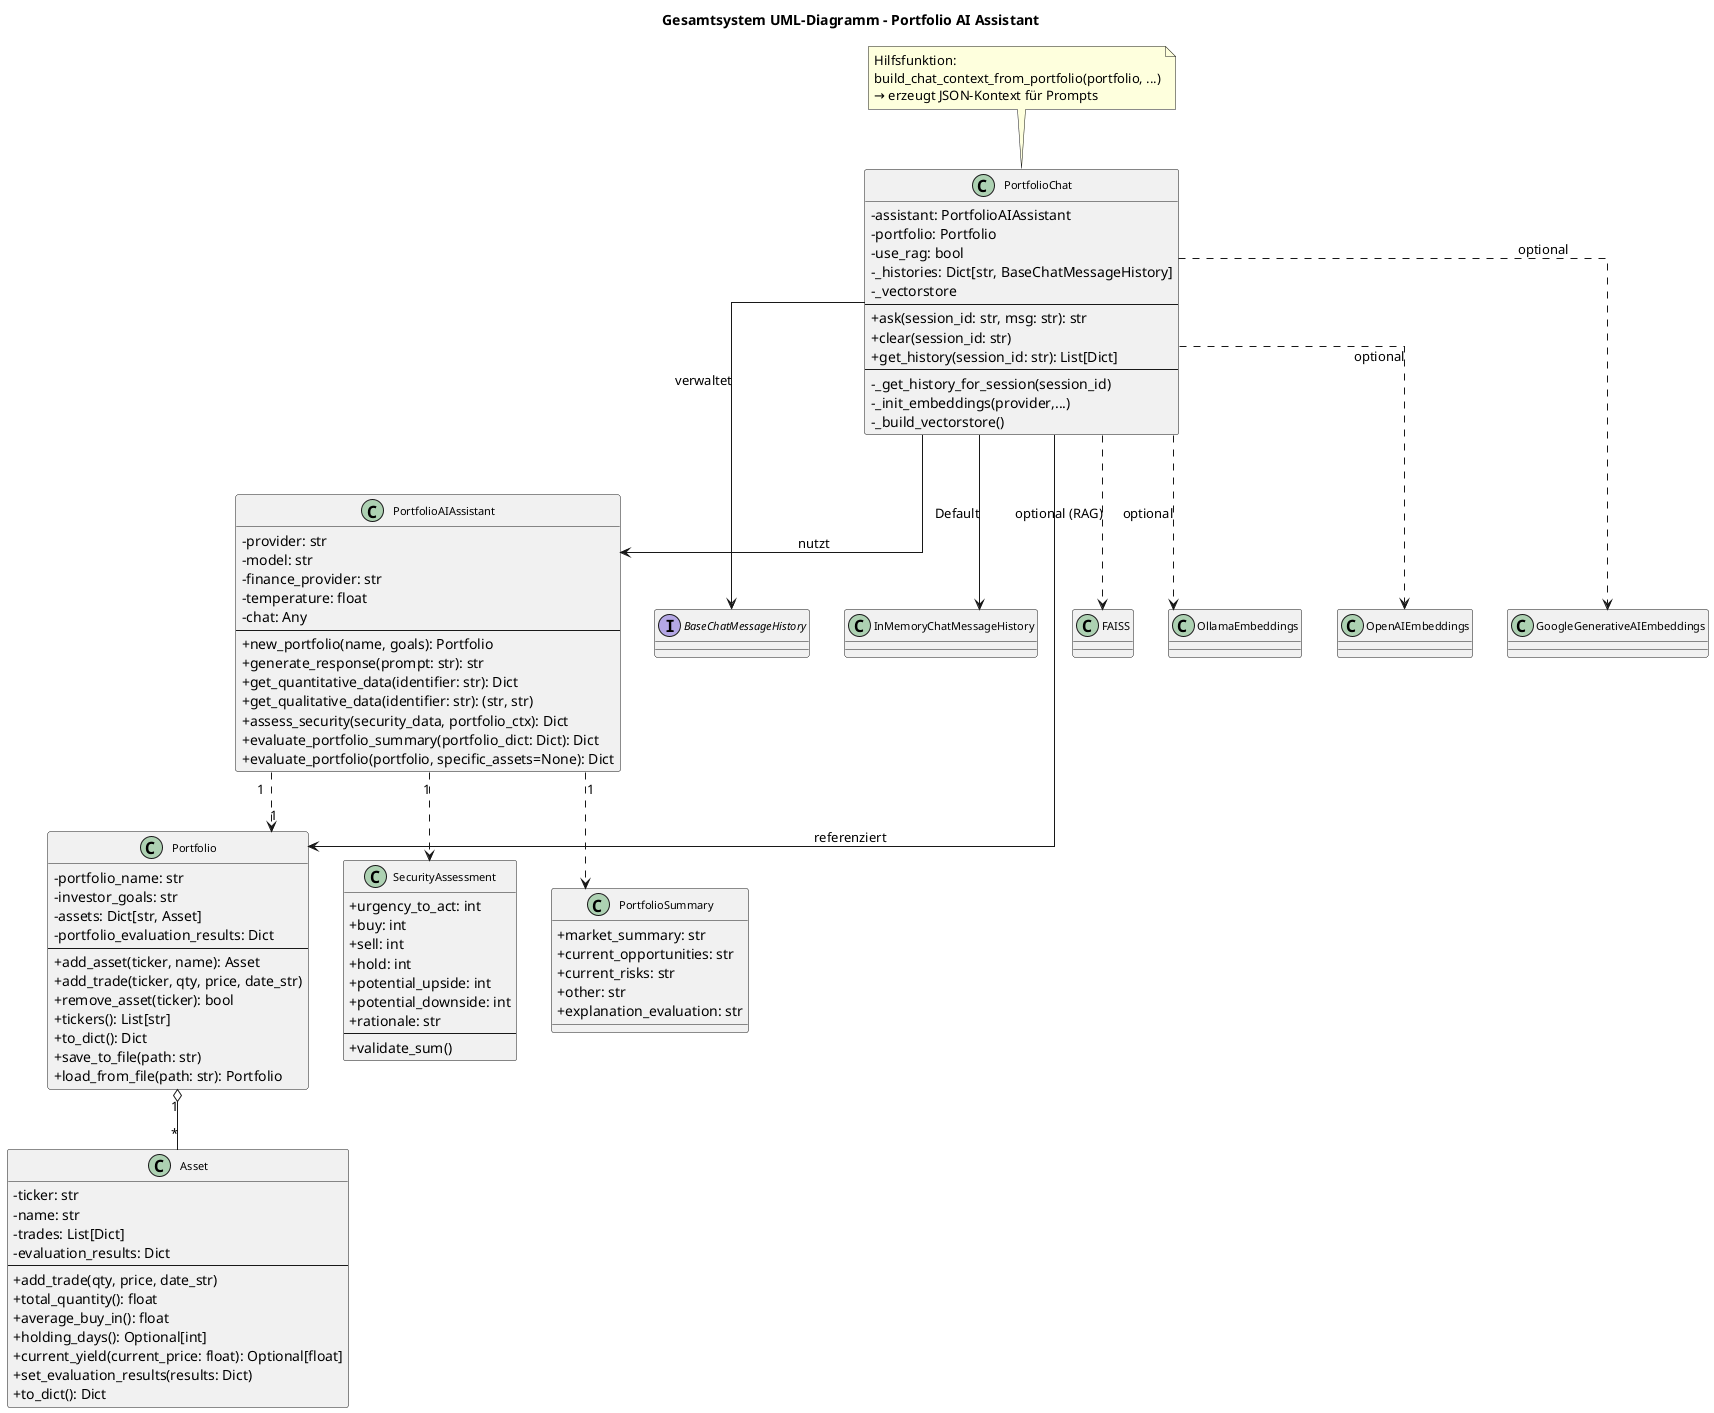
\includegraphics[width=\linewidth]{assets/misc/uml_all.png}
        \caption{Gesamtheitlicheres UML}
    \end{figure}
    }

\tocless\chapter{Flowcharts weiterer Abläufe}
\label{sec:flow_all}

    \tocless{
    \begin{figure}[H]
        \centering
        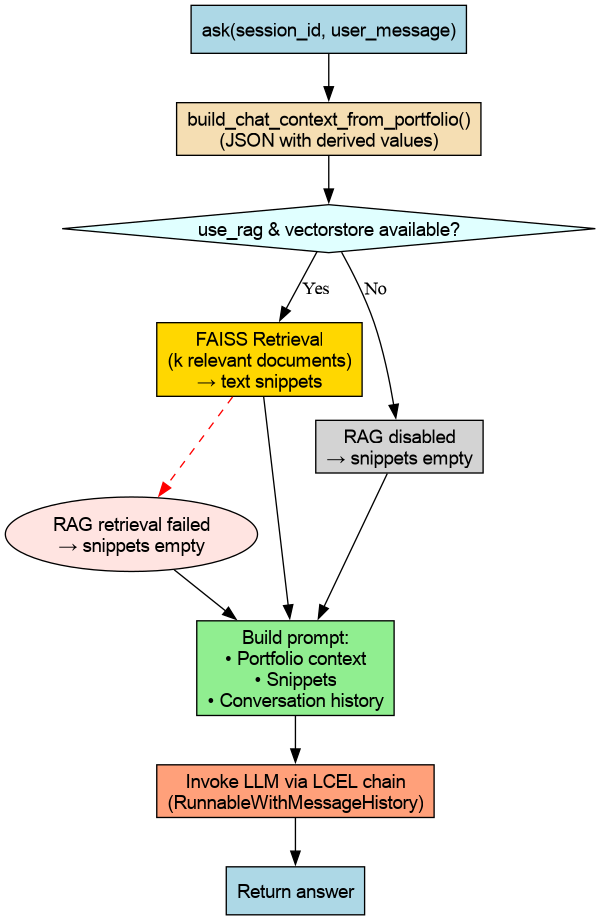
\includegraphics[width=\linewidth]{assets/misc/flowchart_chat.png}
        \caption{Flowchart für Chat-Funktion}
    \end{figure}
    }

\tocless\chapter{Screenshots vom Frontend}
\label{sec:screenshots_frontend}

    \tocless{
    \begin{figure}[H]
        \centering
        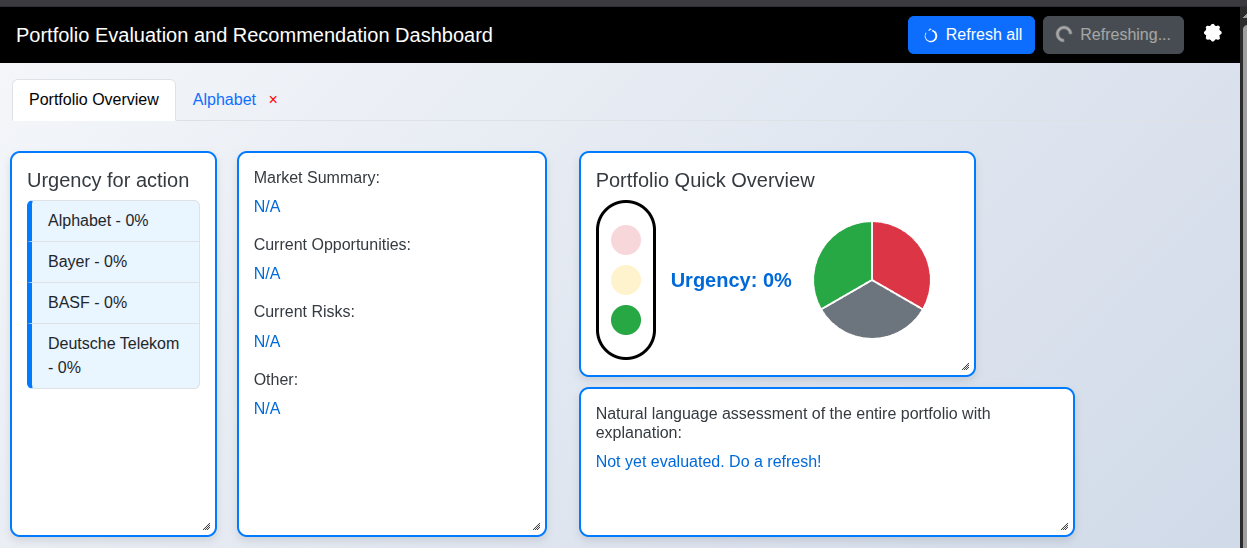
\includegraphics[width=\linewidth]{assets/pictures/screenshot_frontend_vor_evaluierung.png}
        \caption{Frontend in Ausgangssituation vor abgeschlossener Evaluierung mit anderen Wertpapieren}
    \end{figure}
    }

    % To-Do: Bild von Settings, noch mehr Chat, Einzelansichten ...


\tocless\chapter{Ergebnisse von Versuchsaufbauten mit unterschiedlichen Modellen und Optionen}
\label{sec:versuchsaufbau_alternativ}

    \tocless{
    \begin{figure}[H]
        \centering
        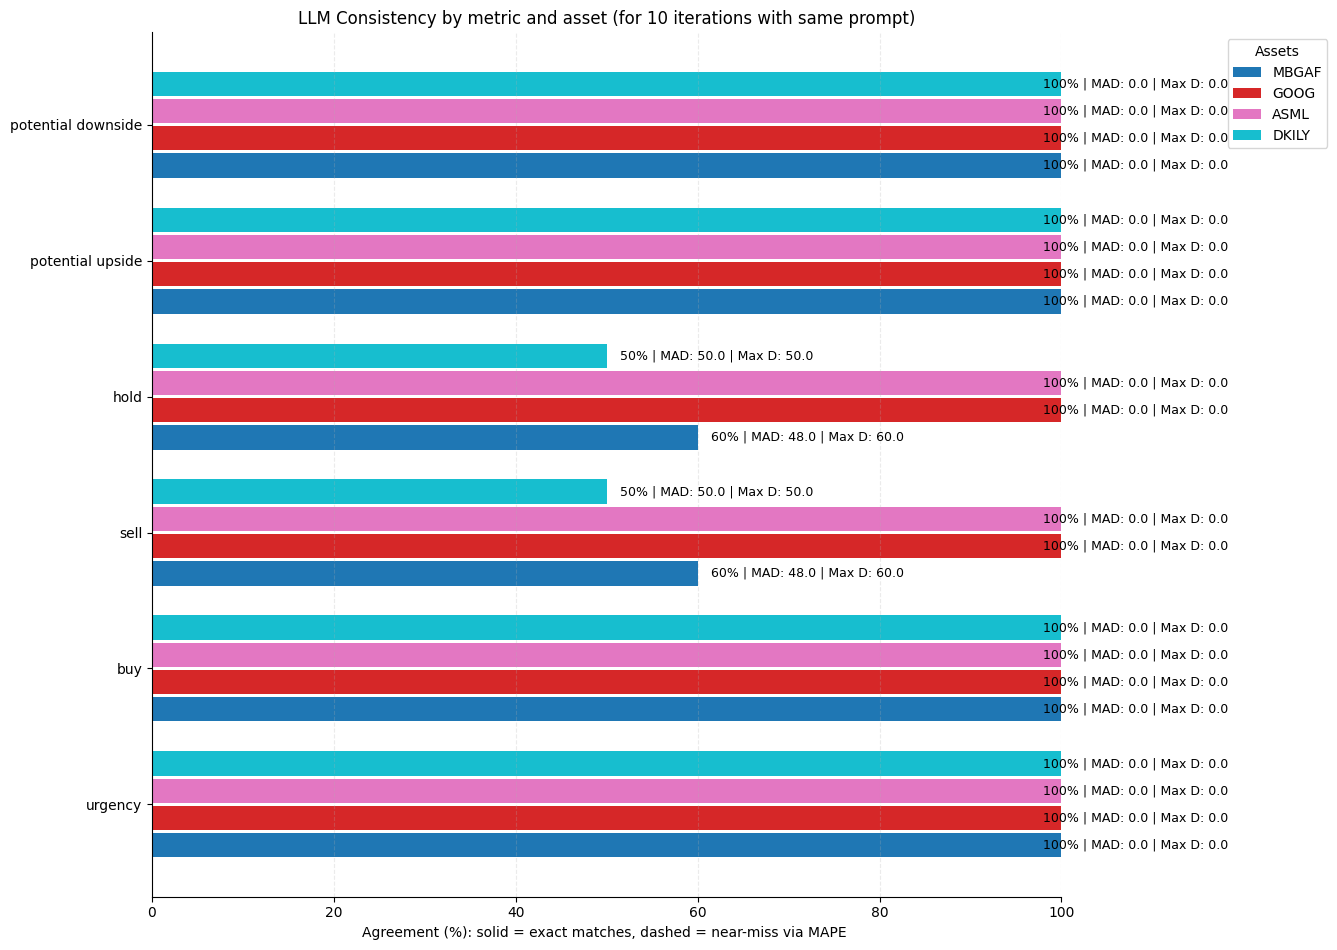
\includegraphics[width=\linewidth]{assets/pictures/evaluation/llm_konsistenz_qwen3_tmp_0_30b_2.png}
        \caption{Ergebnisse des Versuchsaufbaus für die Konsistenzprüfung mit Qwen3:30b und 0.2 als Temperatur}
    \end{figure}
    }

    \tocless{
    \begin{figure}[H]
        \centering
        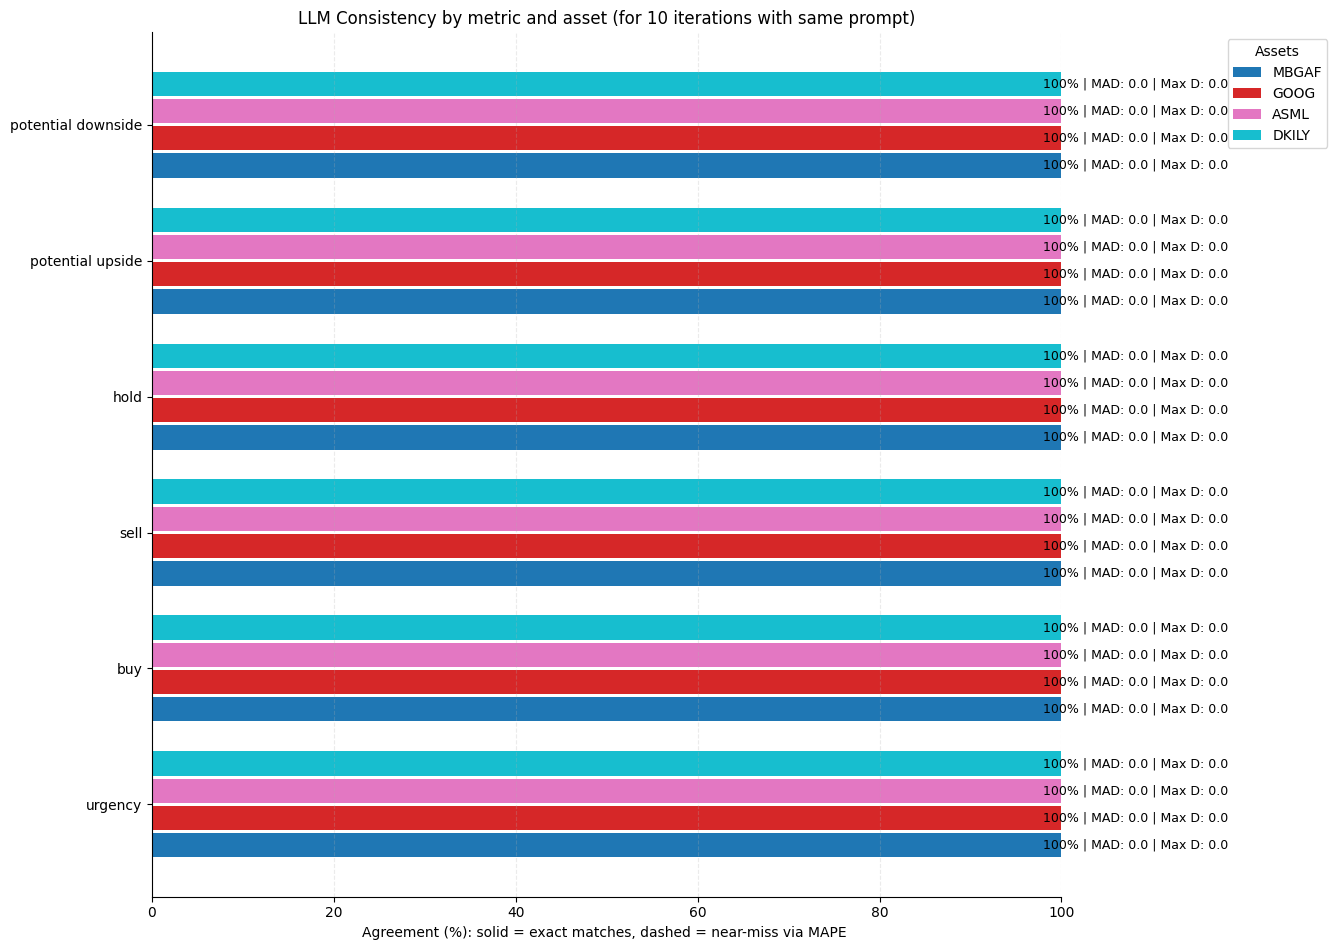
\includegraphics[width=\linewidth]{assets/pictures/evaluation/llm_konsistenz_qwen3_tmp_0_14b.png}
        \caption{Ergebnisse des Versuchsaufbaus für die Konsistenzprüfung mit Qwen3:14b und 0 als Temperatur}
    \end{figure}
    }

    % To-Do: noch mit OpenAI bzw Nexus zeigen ...


\tocless\chapter{Juypter-Lab PDF Export}
\label{sec:jupyter-lab-export}



\tocless\chapter{Code}
\label{sec:full_code}

    % To-Do: Code als lsting einbinden?